\documentclass[../main.tex]{subfiles}
\begin{document}
\renewcommand{\baselinestretch}{1.5}
\chapter{Project Solution}
This chapter consists of the functional- and technical design of the project as a means to resolve the problem statement.

\section{Functional Design}
\subsection{Front end}
\subsubsection*{Login}

The intention for this system was meant to run as an internal site for students and employees, the group choose to remove the register button as one would login with ones existing UiA Login details.\ref{fig:portal_login}
\begin{figure}[H]
    \centering
    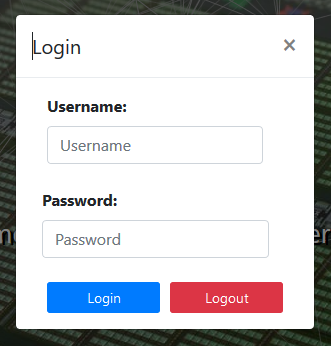
\includegraphics[scale=.7]{img/frontend/portal_login.png}
    \caption{Login modal with login form, for getting access to monitor and request containers}
    \label{fig:portal_login}
\end{figure}


\subsubsection*{Monitoring}
As monitoring containers was an important key in the preliminary report we made a simple page where one could instantly get the status of a container and how much resources a container have been allocated.\ref{fig:portal_monitoring.png}
\begin{figure}[H]
    \centering
    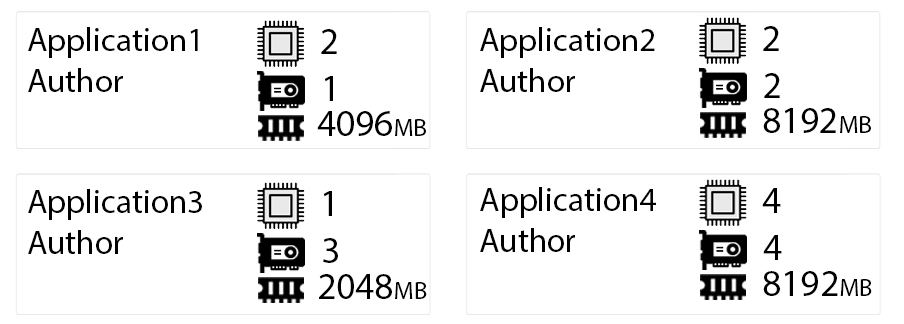
\includegraphics{img/frontend/monitoring_frontend.jpg}
    \caption{Monitoring your personal containers}
    \label{fig:portal_monitoring.png}
\end{figure}


\pagebreak\section{Technical Design}
\subsection{Architecture overview}
The architecture, as shown in figure \ref{fig:architecture_overview}, is set up such that it will have possibilities to scale with increased demand for both compute- and storage capacity. It is flexible enough to allow for up and down scaling of resources, both from a physical infrastructure view as well as allow for individual parts such as the front end application to be scaled to multiple instances or multiple workers if demand increases.
\begin{figure}[H]
    \centering
    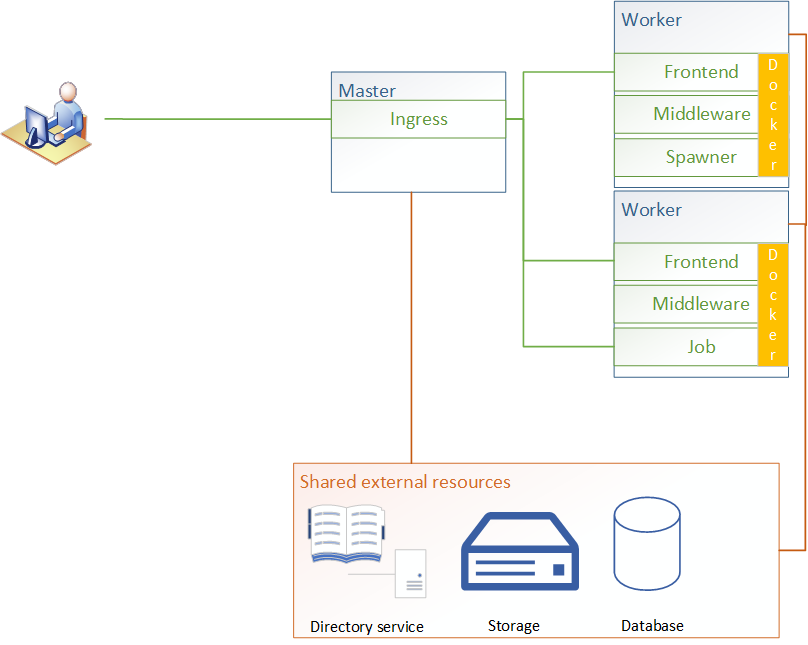
\includegraphics[scale=.75]{img/architecture_overview.png}
    \caption{High level overview of the architecture of the finished design}
    \label{fig:architecture_overview}
\end{figure}
Leveraging the systems themselves and using them for what they are designed for. For example MySQL has clustering capabilities, it is therefore better to let the database itself handle its own clustering and scaling instead of building this into Kubernetes using deployments. Running the database outside the cluster also frees as much resources as possible to the compute jobs on the worker nodes.\\
It is possible to run the master on multiple nodes to ensure high availability, as showing in figure \ref{fig:architecture_overview_lb}, using a third party load balancer to distribute requests. \cite{kubernetes_ha}

\begin{figure}[H]
    \centering
    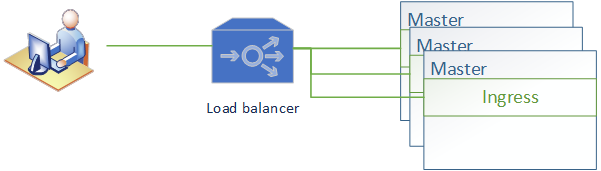
\includegraphics{img/architecture_overview_lb.png}
    \caption{Load balanced master cluster}
    \label{fig:architecture_overview_lb}
\end{figure}



\subsection{Middleware}\label{sec:tech_design_middleware}
% mellomlaget mellom front og kube... 
\subsection*{Authentication flow}
To allow a centralized authentication scheme that can be used with other resources, leveraging existing infrastructure and not having to handle user data in a seperate system, we utilize LDAP. When the user visits the front end he or she will be prompted to provide a username and password to the system, this is then forwarded as a login request to the directory service for validation. If the combination is incorrect the user will not get an access token and as such should not be allowed further onto the system. If the combination is a success, the system will check if the user is part of a valid directory group that is set up for the service, for example "DGX-Users". If this is true, the system will generate an access and refresh token that will be sent back to the user which will be used for further authentication. Figure \ref{fig:authentication_flow} illustrates how the authentication workflow is processed.
\begin{figure}[H]
    \centering
    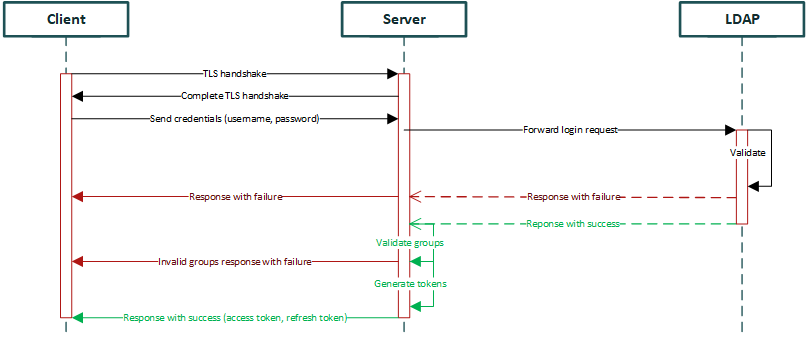
\includegraphics[scale=.75]{img/authentication_flow.png}
    \caption{Authentication flow}
    \label{fig:authentication_flow}
\end{figure}

\pagebreak\subsection*{Job model}
The job model describes how a request for resources should be stored in the database, and what fields are required for future processing. These fields with description can be seen in table \ref{tab:job_model}. It contains information that will be available to the user interface through the API so the user can monitor their requests and get information on how to connect. It also contains information useful for the back end to work with the Kubernetes cluster.
\begin{table}[H]
    \begin{tabular}{|l|l|p{.6\linewidth}|}
        \hline
        \textbf{Field} & \textbf{Type} & \textbf{Value} \\\hline
        id & int & An incremental value assigned by the database \\\hline
        CName & varchar & The canonical name of the job specified by the requester \\\hline
        Author & varchar &  The username of the requester, this is set by the system on creation \\\hline
        CPU & int & The maximum limit of the number of CPU cores, this can not be less than 1 \\\hline
        RAM & int & The maximum limit of the amount of RAM\\\hline
        GPU & int &The number of GPUs requested\\\hline
        Status & int & Specifies the status of the job, see table \ref{tab:status_codes} for more detail\\\hline
        Date created & timestamp & The date and time the request was created \\\hline
        Date modified & timestamp & The date and time the request was last modified \\\hline
        SSH & int & Port number for connection to the container \\\hline
        Jupyter & int & Port number for connection to the Jupyter on the container \\\hline
        Deployment/service prefix & varchar & A string composed of the username-UID which will be the name of the Kubernetes deployment and service names \\\hline
    \end{tabular}
    \caption{The definition of the job model to be stored in the database}
    \label{tab:job_model}
\end{table}


\begin{table}[H]
    \centering
    \begin{tabular}{|l|l|}
    \hline
        \textbf{Code} & \textbf{Description} \\
        \hline
        0 & Stopped \\
        \hline
        1 & Running \\
        \hline
        2 & Pending restart \\
        \hline
        3 & Pending stop \\
        \hline
        4 & In queue \\
        \hline
    \end{tabular}
    \caption{The status codes of the queue model}
    \label{tab:status_codes}
\end{table}
When information for a job or all jobs for the user is requested, or a new job is put on the queue successfully, a JSON formatted object will be returned containing details for the front end to display, a sample request is shown in figure \ref{fig:middleware_job}.
\begin{figure}
    \centering
    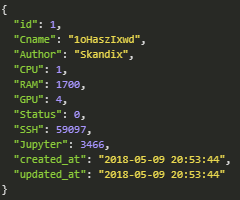
\includegraphics{img/middleware_job.PNG}
    \caption{Shows an example of a JSON object of a job returned from the middleware}
    \label{fig:middleware_job}
\end{figure}

\pagebreak\subsection*{Middleware API routes}
The back end contains two controllers
\begin{itemize}
    \item AccountController\\
            Handles routes for login and logout
    \item QueueController\\
            Handles routes related to issuing and retrieving job requests
\end{itemize}
The controller endpoints can be seen in table \ref{tab:api_endpoints}
\begin{table}[H]
    \centering
    \begin{tabular}{|l|l|}
        \hline\textbf{Route} & \textbf{Description}  \\\hline
        /account/login & Issues a valid token on success full login\\\hline
        /account/logout & Deauthorizes the token \\\hline
        /queue & Retrieves all the items in the queue for the logged in user\\\hline
        /queue/{id} & Retrieves a specific item for the queue for the logged in user \\\hline
        /queue/create & Post a new job request \\\hline
        /queue/stop/{id} & Request that the job be stopped \\\hline
        /queue/restart/{id} & Request a restart of the job \\\hline
    \end{tabular}
    \caption{Available API endpoints}
    \label{tab:api_endpoints}
\end{table}


\subsection*{New job request}
The processing of a new job request to be put on the queue starts with checking the validity of the token, this is to ensure that even if you know the route one should not be able to post requests. Once authorization is confirmed, the input data should be validated against a rule set as defined in table \ref{tab:basic_ruleset}

\begin{table}[H]
    \centering
    \begin{tabular}{|l|p{0.8\linewidth}|}
        \hline\textbf{Field} & \textbf{Rule set} \\\hline
        CName & Should be a string, of maximum length 255 \\\hline
        CPU & Should be an integer, a minimum and maximum size should be proportionate to the average server in the cluster \\\hline
        RAM & Should be an integer, a minimum and maximum size should be proportionate to the average server in the cluster \\\hline
        GPU & Should be an integer, of value 0 to a maximum that should be proportionate to the average server in the cluster \\\hline
    \end{tabular}
    \caption{The basic rule sets for the input fields when requesting a new job from a high level}
    \label{tab:basic_ruleset}
\end{table}
Given the unknown nature of the jobs to be queued the limits should be flexible enough to allow multiple jobs to be running at the same server, while at the same time not be to strict with regards to user requirements. This needs approval and discussion within the organization, and should be accepted from the top of the chain.\\
The request should then have the author, status and time stamps appended before being stored in the database for further processing. Finally the endpoint should return a JSON object with the registered information to the front end. The flow of this procedure is shown in figure \ref{fig:middleware_new_request}

\begin{figure}[H]
    \centering
    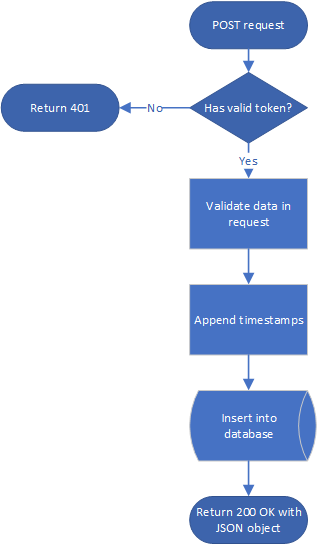
\includegraphics{img/middleware_new_request.png}
    \caption{New request processing at a high level}
    \label{fig:middleware_new_request}
\end{figure}


\subsection*{Getting jobs for the user}
The processing of getting jobs starts with checking the validity of the token. This is to ensure that only a valid user can retrieve their own jobs and not the jobs of someone else. If the token is invalid we immediately return a 401 Unauthorized. This also has the side effect that trying to probe for valid job id's will net a 401 no matter if the id is valid or not.\\
The process then retrieves all jobs for the user and formats it into a JSON object, which is returned to the front end. This process can be seen in figure \ref{fig:middleware_get_jobs}
\begin{figure}[H]
    \centering
    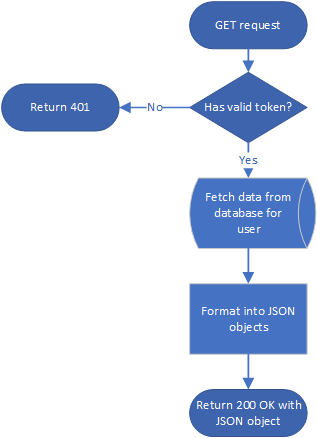
\includegraphics{img/middleware_get_jobs.png}
    \caption{Fetching all jobs in queue for the user from a high level}
    \label{fig:middleware_get_jobs}
\end{figure}
The process of getting a single job is equivalent in its process, as seen by figure \ref{fig:middleware_get_single_job}

\begin{figure}[H]
    \centering
    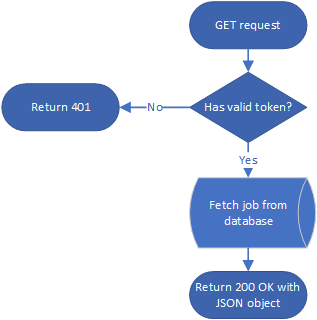
\includegraphics{img/middleware_get_single_job.png}
    \caption{Fetch a specific job for the user from a high level}
    \label{fig:middleware_get_single_job}
\end{figure}

\subsection*{Restart or stop job by id}
The process of restarting or stopping a specific job starts by validating the token, this is to ensure that only a valid user can update his or her job. If the token is invalid it should return 401 Unauthorized immediately. Then verifying the existence of the job in the database, and subsequently updating with the correct status code as given in table \ref{tab:status_codes}. Data changed should also be updated to reflect the time of the action. Finally the edited job is returned as a JSON object. The process can be seen in figure \ref{fig:middleware_change_status}.
\begin{figure}[H]
    \centering
    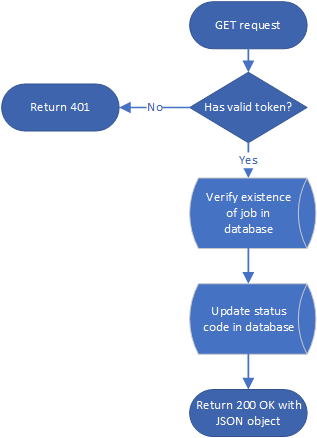
\includegraphics{img/middleware_change_status.png}
    \caption{Update the status code as requested by user on restart or stop request from a high level}
    \label{fig:middleware_change_status}
\end{figure}




\subsection{Queue Manager}
% Den som spawner containere, restarter etc.
The queue manager's job is to respond to requests in the queue. This entails creation, restarting and removing of deployments in Kubernetes. It is running as a single entity to ensure that we do not have concurrency issues. The workload should be light enough that a single instance is sufficient. Running separately from the middleware this also ensures that should one get unauthorized access to the middleware layer, this does not give you any access to the Kubernetes cluster. A high level overview can be seen in figure \ref{fig:automation_timed_flow}.
\begin{figure}
    \centering
    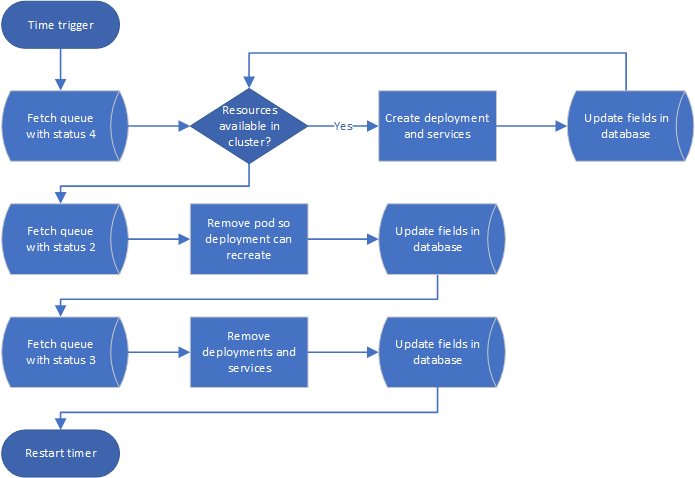
\includegraphics{img/automation_timed_flow.png}
    \caption{Timed creation, restart, stop of deployments for the work requests from a high level}
    \label{fig:automation_timed_flow}
\end{figure}
The queue manager will run on a timed trigger, for example every 5 minutes to process the queue.
\subsection*{New requests}
The queue manager will query the database for all jobs that are new sorted from oldest to newest based on created time stamp. Given the impression of a relaxed workload, this will work as a FIFO queue. Based on the specifications of the first job it will check if any worker node in the cluster has enough resources available, if not enough resources are available then it is done.\\
If resources are available it will create a deployment based on the specifications and push this to Kubernetes. This will ensure that the pod will be recreated should the current working node go down or the pod be killed by some other means. It will also create a service endpoint so SSH and Jupyter can be reached from outside the cluster. Finally it will update the fields in the database with the prefix of the deployment and service in accordance with table \ref{tab:job_model}.\\\\
The drawback with using the FIFO queue model, is that a single job, that requires all the GPU capacity of a worker node, can block all other requests. As such an implementation of weighted fair queuing can alleviate this to some extent by weighing based on resource specification by setting a limit on what is a "fair" amount of resource usage. One can then prioritize getting smaller jobs through by treating for instance 0 to 4 GPUs as fair. This has business implications and does need more analysis based on usage patterns as well as discussion and approval from CEO level.

\subsection*{Restart requests}
This will query the database and retrieve all jobs with the restart status code, using the prefix it then identifies the correct deployment and can then get access to the specific pod that the job is running under. Deleting the pod, Kubernetes will attempt to do a graceful shutdown, and then recreate the pod. Finally it will then update the status in accordance with table \ref{tab:status_codes} and changed time stamp field in the database.

\subsection*{Stop requests}
This will query the database and retrieve all jobs with the stop status code, using the prefix it then identifies and removes the correct deployment and services from Kubernetes. Finally it updates the status code in accordance with table \ref{tab:status_codes} and changes the changed time stamp field in the database.


\subsection{Kubernetes}
\subsection*{Master}
The master node is responsible for managing the cluster, and distributing the jobs across the worker nodes. Using docker through official channels, it is set up with flannel for in-cluster routing, kube-dns for namespace resolution inside the cluster, as well as applying the feature set to schedule GPU resources.
%\inputminted[linenos, breaklines]{bash}{code/kubernetes.master.sh}


\subsection*{Worker without GPU}
A worker without GPU requirements only requires docker from the official channels, as well as the kubelet and kubeadm services.\\
Using \mintinline{vim}|kubeadm join --token <token> --discovery-token-ca-cert-hash <hash>| to join the cluster, the master will automatically assign required infrastructure to fulfill requirements. The tokens by default only have a 24 hour lifespan, as such it is required to create a new token on the master node, the simplest way is \\
\mintinline{vim}|kubeadm token create --print-join-command|, one can append \mintinline{vim}|--ttl <duration>| in the format of XhYmZs, if the value is 0 it will never expire. \cite{kubeadm_token}
\begin{figure}[H]
    \centering
    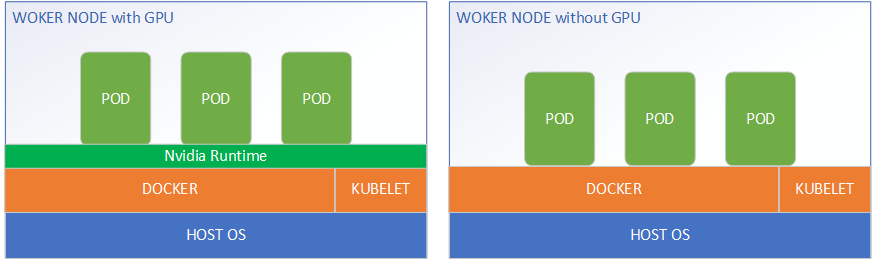
\includegraphics{img/Kubernetes_individual_nodes.png}
    \caption{Worker nodes with software components installed, both with and without a GPU resource to be used}
    \label{fig:kubernetes_individual_nodes}
\end{figure}

\subsection*{Worker with GPU}
A worker with GPU requires the installation of a compatible driver, testing has shown version $\geq$ 390 works, as well as CUDA drivers. To leverage NVIDIA-docker the Docker community edition has to be used and NVIDIA has to be set as the default runtime for Docker. Upon joining the cluster as described in "Worker no GPU" the master will assign the required infrastructure to fulfill requirements.

\subsection*{Ingress}
The ingress is responsible for forwarding requests to the front end of the application from outside the cluster using a Kubernetes ingress control pointing to a Kubernetes service. This ensures that the deployment of the front end application can be replicated over multiple hosts as demand increases, and the service is responsible for identifying and forwarding to running pods.

\subsection*{Jupyter and SSH access}
Through the usage of Kubernetes nodeport service requests can be forwarded based on the port number to a pod.


\subsection{Shared external resources}
\subsection*{Shared storage}
To enable independence of which host the job will be run at, a shared external storage should be used. This is due to the size of training data for AI purposes can be quite large, thus having to replicate this to every node is not feasible. This further allows the administrator an easy to manage storage infrastructure that can be scaled separately from Kubernetes.\\
As such NFS can be leveraged through a shared storage network that is separate from the cluster, using a path name scheme such as \mintinline{bash}|/storage/share/<username>| will allow definition of NFS mount points to only mount the requester' structure as volume on the created pod.


\subsection*{Database}
The database is responsible for storing the queue information. This can be run inside the cluster, but it is recommended to run outside. This is to leverage the database platform itself to have a distributed system, and so it can scale independently of Kubernetes. As well as freeing more resources to process job requests.

\subsection*{Authentication}
Since the a deployment will happen in an existing environment, there is no need for an independent system of user names and passwords. As such leveraging the abilities through LDAP to access directory services outside of the cluster will ensure availability and easier user management through the usage of group assignments for authorization into the system.\\
Through an API endpoint authentication is performed, and an access token is generated for the session which is then used for authorization to the queue endpoints as described in the section \ref{sec:tech_design_middleware}


\subsection{Monitoring}
\begin{figure}[H]
    \centering
    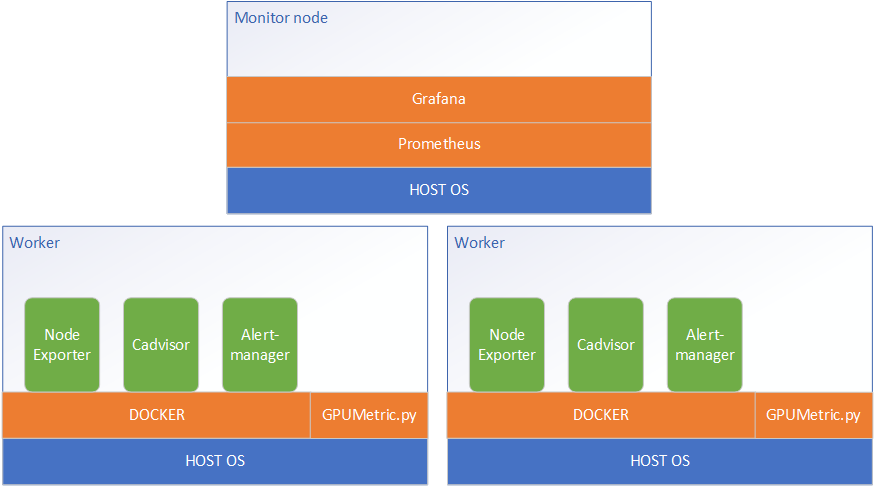
\includegraphics[scale=0.8]{img/Monitoring_stack.png}
    \caption{An overview of the monitoring stack}
    \label{fig:Monitoring_stack}
\end{figure}
The group managed to get most of the monitoring working for both dockers and the GPU. Each of the services below is ran in Docker containers, and is managed with Docker compose. Due to that all of the services need to communicate with each other it is needed that all of them would start at the same time as well as it makes everything a lot easier to manage when its supposed to be deployed on multiple nodes. However the GpuMetric script would not be running in a Docker container as it would occupy all the GPUs on the system as a GPU can only be allocated once. This would mean that it had to be ran with a service manager such as systemd \cite{systemd} or systemctl \cite{systemctl}. 

\subsection*{GpuMetric}
GpuMetric is a python script written by the group to gather information about the NVIDIA specific GPU's and push it to a text file, which then can be imported by the Prometheus \cite{prometheus} node-exporter \cite{nodeexporter}. GpuMetric is  using a python library py3nvml \citep{py3nvml} to gather specific information such as temperature, memory- and power usage  about the graphics cards on the host.   %  MARKER JAIL %

\subsection*{Node Exporter}
Node Exporter is part of Prometheus and it is in command of ensuring to collect information about the host.

\subsection*{Alertmanager}
Alertmanager \cite{alertmanager} is part of Prometheus, and its purpose is to handle the alarms that is being sent from Prometheus. 

\subsection*{Cadvisor}
Container Advisor \cite{cadvisor} is a tool made by Google to collect live metrics from running containers. % får fylle litt mer på her etterhvert 

\subsection*{Prometheus}
Prometheus is a time-series database and a powerful monitoring tool. It has multiple integration points as well as an efficient way of storing data.

\subsection*{Grafana}
Grafana is a highly customizable dashboard for analyzing and monitoring data both real time and historical data. It also support multiple data sources like here we are using Prometheus to point out one of the most popular ones. 

\end{document}